\chapter{\MakeUppercase{Conceptos generales del problema oncológico de crecimiento tumoral de un tumor avascular y fundamento matemático para el estudio de este problema}}
%\chapter{Conceptos generales del problema oncológico de crecimiento tumoral de un tumor avascular y fundamento matemático para el estudio de este problema}
\thispagestyle{fancy}
\section{Conceptos acerca del tumor avascular}

Las células del cuerpo humano normalmente tienen un  crecimiento controlado y limitado a tejidos específicos, sin embargo en algunos casos la división celular se vuelve desordenada e invade diferentes tejidos, esta enfermedad es llamada cáncer. En ocasiones el proceso de división celular da lugar a tumores, estos pueden ser malignos o benignos dependiendo si las células de tumor invaden otras partes del cuerpo o no.

En el año 2020, el cáncer en todas sus formas fue responsable de 10 millones de muertes a nivel mundial \citep{Revilla2021} y es la segunda causa de muerte en el continente americano.

En el Perú anualmente se detectan un aproximado de 70000 casos nuevos de cáncer y casi 35000 personas mueren por causa del cáncer. Se proyecta que para el año 2040 se realicen 123000 diagnósticos mientras que el número de fallecidos ascienda a 65000 \citep{cancertomorrow}.


%
%https://ourworldindata.org/explorers/coronavirus-data-explorer?facet=none&Metric=Confirmed+deaths&Interval=Cumulative&Relative+to+Population=false&Color+by+test+positivity=false&country=~OWID_WRL
%Variable time span	Jan 22, 2020 – Sep 23, 2022
%Data published by	COVID-19 Data Repository by the Center for Systems Science and Engineering (CSSE) at Johns Hopkins University
%Link	https://github.com/CSSEGISandData/COVID-19
%
%Raw data on confirmed cases and deaths for all countries is sourced from the COVID-19 Data Repository by the Center for Systems Science and Engineering (CSSE) at Johns Hopkins University.
%
%Our complete COVID-19 dataset is a collection of the COVID-19 data maintained by Our World in Data. It is updated daily and includes data on confirmed cases, deaths, hospitalizations, and testing.
%
%You find it at our GitHub repository here.

La mayoría de los diagnósticos se dan en una etapa avanzada del cáncer y por eso el alto indice de mortalidad, por lo tanto el diagnóstico y tratamiento temprano son de suma importancia. 

El crecimiento tumoral admite dos etapas importantes: la etapa avascular, donde los nutrientes son  absorbidos por la frontera del tumor, y la etapa vascular donde el tumor genera su propia red de vasos sanguíneos a través e un proceso conocido como angiogénesis, para finalmente llegar a invadir tejidos sanos en otras partes del cuerpo (metástasis). La transición entre la etapa avascular y la etapa vascular se da principalmente cuando el tumor excede un diámetro critico del orden de 2 mm, ya que los nutrientes absorbidos del entorno son insuficientes para continuar con el crecimiento del tumor y comienzan a secretar sustancia químicas que por difusión alcanzan tejido vascular para formar una nueva red de alimentación de nutrientes, esta etapa toma aproximadamente de 10 a 21 días \citep{macklin2009multiscale}, por lo que analizar el crecimiento del tumor en la etapa avascular es clave para un tratamiento temprano.

%\subsection{Descripción del tumor avascular}

Los tejidos donde se desarrolla un tumor presenta las siguientes etapas de formación:
\begin{itemize}
	\item Hiperplasia: se caracteriza por el rápido aumento del número de células en el tejido afectado. Las células tiene una apariencia normal y en general esta etapa es benigna.
	\item Displasia: el crecimiento celular se vuelve descontrolado y la estructura del tejido cambia por la malformación celular. Un ejemplo son los lunares de borde irregular.
	\item Carcinoma ``in situ'': se considera así a un tumor pre canceroso con crecimiento casi autónomo pero que no ha iniciado la etapa invasiva.
\end{itemize}
Durante la etapa avascular el tumor obtiene nutrientes por difusión a través de la frontera y su crecimiento ocurre por mitosis celular hasta que la densidad de células malignas en un volumen especifico llega a ser tan alta que son desplazadas a áreas menos comprimidas donde continua la división celular. 

%\subsection{Importancia del tumor avascular}

Entre los modelos existentes podemos mencionar 
\begin{enumerate}
	\item Modelos microscópicos, son modelos discretos basados en autómatas celulares
	\citep{interian2017tumor}. 
	\item Modelos macroscópicos, son modelos continuos basados en ecuaciones diferenciales parciales \citep{mantilla2010}.
\end{enumerate}
\section{Fundamento matemático}
El modelamiento de procesos biológicos y físicos donde una curva de nivel representa la frontera entre dos medios, ha sido  llevado a cabo de diversas maneras:
\begin{itemize}
	\item En \citep{mantilla2010} se resuelve el modelo de crecimiento tumoral restringido a una frontera circular por medio del Método de Elementos Finitos (FEM) con penalización y con curvatura calculada por medio del Método de Diferencias Finitas (MDF).
	\item En \citep{dinh2018finite} se resuelve un modelo de crecimiento de colonias de microorganismos  por medio del Método de Elementos Finitos Extendidos (NXFEM) y estabilización de la evolución de la frontera. 
	\item  En \citep{macklin2005evolving} se resuelve el modelo de crecimiento tumoral por medio del Método de Diferencias Finitas (MDF) con estabilización de la velocidad por medio de un filtro gaussiano.		\item  En \citep{calzada2011fictitious} se resuelve el modelo de crecimiento tumoral por medio del Método de Elementos Finitos y multiplicadores de Lagrange con estabilización de la evolución de la frontera con un método WENO de quinto orden y el método de Runge-Kutta de tercer orden. Un método WENO (\emph{Weighted Essentially Non-Oscillatory}) consiste en reducir las oscilaciones cerca a una discontinuidad por medio de una combinación convexa de polinomios de Lagrange  \citep{hang2021conservative}.
	
	\item  En  \citep{shopple2009interface} se resuelve un modelo de solidificación medio del Método de Elementos Finitos con refinamiento de malla en la frontera, la cual es aproximada por segmentos rectos. 
\end{itemize}
\section{Representación de la frontera del tumor}
La frontera del tumor puede ser representada por un conjunto de aristas de un mallado triangular o por medio de una curva de nivel definida en dominio triangulado de manera uniforme.
\begin{figure}[H]
	\centering\hfil
	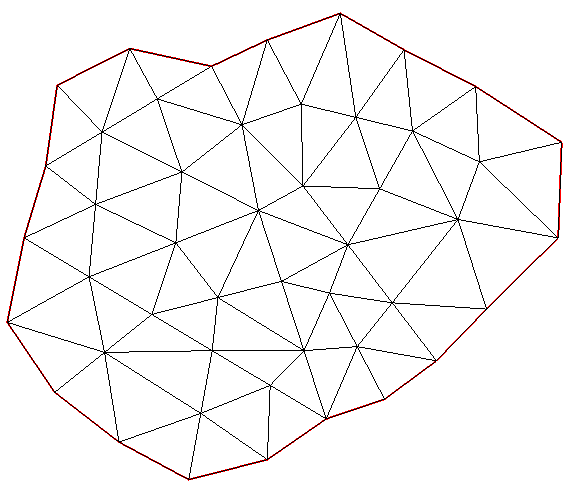
\includegraphics[width=0.4\linewidth]{img/mallaajustadafronteranorefinada}\hfil	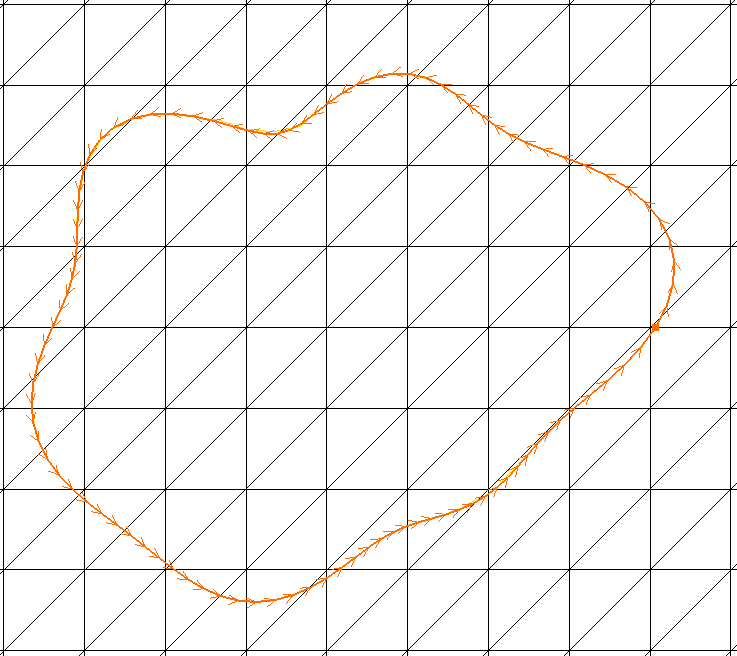
\includegraphics[width=0.4\linewidth]{img/mallanoajustadafrontera}
	\caption{Representación de la frontera. Izquierda: Frontera representada por segmentos rectos. Derecha: Frontera representada por curva de nivel.}
	\label{fig:mallanoajustadafrontera}
\end{figure}
La representación de la frontera ajustada al mallado trae dificultades en el cálculo de la curvatura, además exige que la malla cambie en cada paso de tiempo y por lo tanto la solución numérica debe interpolarse a la nueva malla. La representación por curvas de nivel permite el uso de polinomios de grado 2 y 3, ademas de eliminar la necesidad de cambiar la malla.

Entre los métodos numéricos que utilizan un malla fija y permiten que la frontera o interface cruce los elementos,  se encuentran:
\begin{itemize}
	\item El Método de Elementos Finitos Extendidos (XFEM), basado en enriquecer los elementos interceptados por la interface, con  funciones de forma discontinuas y fue utilizado por primera vez para resolver problemas de propagación de fracturas \citep{olsson2005conservative}. La estabilización se logra desactivando  grados de libertad, por precondicionamiento o mediante el uso de penalidad fantasma.
	\item El Método de Elementos Finitos Cortados (CutFEM)  por otra parte utiliza dominios ficticios en combinación con penalidad fantasma para estabilizar la solución, ha sido utilizado principalmente en problemas de flujos bifásicos \citep{claus2019cutfem}.
	
	\item El Método de Elementos Finitos basado en Conjuntos de Nivel ($\phi$-FEM), presentado en \cite{duprez2020phi}-\cite{cotin2021phifem}  utiliza funciones forma que se anulan en la curva de nivel 0, que representa la frontera, ha sido utilizado en problemas de transferencia de calor y el estudio del	movimiento de partículas rígidas en un fluido regido por las ecuaciones de Stokes.
	\item El Método de Elementos Finitos aplicado a inecuaciones variacionales presentado en \cite{mantilla2003} considera analizar el comportamiento del flujo laminar de un líquido que se filtra a través de una sección transversal de un medio poroso donde la interface entre la región húmeda y la región seca se representa por medio de $q$ una función característica.
	\begin{figure}[H]	
		\centering
		\includegraphics[width=10cm]{img/Zhzsdr.pdf}
		\caption{\label{drsh2b} Filtración en un medio poroso, la frontera que 
			separa la región húmeda y la región seca es representada por una función característica \cite{mantilla2003}.}
	\end{figure}
\end{itemize}
\section{Notaciones}
%Presentamos las siguientes notaciones \citep{brenner2008mathematical}: Sea $\alpha=\left(\alpha_1,\ldots,\alpha_d\right)\in\mathbb{N}^d$  un multi-índice con longitud $|\alpha|=\alpha_1+\cdots +\alpha_d$, entonces $D^\alpha =\left( \partial / \partial x_1\right)^{\alpha_1}\cdots \left( \partial / \partial x_d\right)^{\alpha_d}$. Denotamos por $C^k(\Omega)$ a la clase de funciones en $\Omega$  con derivadas parciales de orden $k$ continuas en $\Omega$, $C_0^k(\Omega)$ denota el conjunto de funciones en $C^k(\Omega)$ con soporte compacto en $\Omega$. Dado $p\in\left [1,+\infty\right>$, $L^p(\Omega)$ denota el espacio de funciones reales $f$ tal que $|f|^p$ es integrable en $\Omega$ respecto a la medida de Lebesgue en $\mathbb{R}^d$. $L^p(\Omega)$ es un espacio de Banach con la norma
%\[
%\|u\|_{L^p(\Omega)} =\left(\int_\Omega |u|^p\right)^{1/p}
%\]
%Ademas $L^2(\Omega)$ es un espacio de Hilbert con el producto interno y norma siguientes
%\[
%\left(u,v\right) = \int_\Omega uv,\quad \|u\|=
%\left(u,u\right)^{1/2}
%\]
%El espacio de funciones con $W^{m,p}(\Omega)$ 
%\[
%\begin{aligned}	
%\|u\|_{m,p} & = \left( \sum_{0\leq|\alpha| \leq m} \| D^\alpha u\|^p_{L^p(\Omega)}\right)^{1/p},\quad 1\leq p <+\infty\\
%\|u\|_{m,\infty} & = \max_{0\leq|\alpha| \leq m} \| D^\alpha u\|_{L^\infty(\Omega)}
%\end{aligned}
%\]
%y las seminormas
%\[
%\begin{aligned}	
%	|u|_{m,p} & = \left( \sum_{|\alpha| = m} \| D^\alpha u\|^p_{L^p(\Omega)}\right)^{1/p},\quad 1\leq p <+\infty\\
%	|u|_{m,\infty} & = \max_{|\alpha| = m} \| D^\alpha u\|_{L^\infty(\Omega)}
%\end{aligned}
%\]
%\end{itemize}
%

Introducimos la notación de multi-índice$\,$para el cálculo de
derivadas parciales. Un multi-índice, $\alpha $, es una d-dupla de
enteros no-negativos, $\alpha _{i}$. La ``longitud'' de $\alpha $ está
dada por $\left| \alpha \right| :=\sum\limits_{i=1}^{d}\alpha _{i}.$ Con
esta notación si $v\in \mathbf{C}^{m}\left( \Omega \right) $ entonces
para cualquier $\alpha $ con $\left| \alpha \right| \leqslant m$,
\[
D^{\alpha }v\left( x\right) =\frac{\partial ^{\left| \alpha \right| }v\left(
	x\right) }{\partial x_{1}^{\alpha _{1}}\cdots\partial x_{d}^{\alpha _{d}}}
\]
es la derivada parcial de $\alpha ^{th}$ orden. Por ejemplo
\[
\frac{\partial v}{\partial x_{1}}=D^{\alpha }v\text{ para }\alpha =\left(
1,0,\ldots,0\right)
\]
\[
\frac{\partial ^{d}v}{\partial x_{1}\cdots\partial x_{d}}=D^{\alpha }v\text{
	para }\alpha =\left( 1,1,\ldots,1\right)
\]

En lo que sigue $\Omega $ designa un conjunto abierto en $\mathbb{R}^{d}$
con frontera $\Gamma $ y se consideran los espacios $\mathbf{L}^{p}\left(
\Omega \right) $, $1\mathbf{\leqslant }p\mathbf{\leqslant }\infty $, dotados
de la medida de Lebesgue $d$-dimensional. $\mathbf{C}_c(\Omega)$ es el espacio de funciones continuas en $\Omega$ con soporte compacto en $\Omega$, es decir se anulan fuera de algún compacto $K\subset \Omega$.

Para un entero $k>0$ definimos los siguientes conjuntos de funciones: $\mathbf{C}_c^k(\Omega)=\mathbf{C}^k(\Omega) \cap \mathbf{C}_c(\Omega)$.
$\mathbf{C}_c^\infty(\Omega)=\mathbf{C}^\infty(\Omega) \cap \mathbf{C}_c(\Omega)$.

\begin{defi}
	Definimos el conjunto $\mathbf{L}_{loc}^{p}(\Omega )$\ para $1\mathbf{%
		\leqslant }p\mathbf{\leqslant }\infty $ y $\Omega \subset \mathbb{R}^{d}%
	\mathit{\ }$como el conjunto de funciones $f$\ tales que:
	\[
	f\in \mathbf{L}^{p}(K)\quad \forall \text{compacto }K\subset \Omega
	\]
\end{defi}

Un ejemplo de función localmente $p$-integrable es
\[
f\left( x\right) =\exp \left( d\left( x,\Gamma \right) ^{-1}\right) \sen%
\left( d\left( x,\Gamma \right) ^{-1}\right)
\]
Así tomando $K\subset \Omega $, $K$ compacto tenemos que existe
$\delta >0$ tal que $d\left( x,\Gamma \right) \geqslant \delta $
para todo $x\in K$ por
tanto $f\left( x\right) $ es continua en $K$ y en consecuencia $p$%
-integrable en $K$. Pero claro $f\left( x\right) \rightarrow +\infty $
cuando $d\left( x,\Gamma \right) \rightarrow 0$.
%\begin{teo}[Urysohn]
%	\label{Teo_Ury}Sea $G\subset \mathbb{R}^{d}$\ un abierto y $K\subset G$\ un
%	conjunto compacto, entonces existe $f\in \mathbf{C}_{c}\left( G\right)$
%	tal que
%	\begin{enumerate}
	%		\item  \hspace{3cm} $0\leqslant f\left( x\right) \leqslant 1\quad\text{
		%			para todo }x\in G$
	%		\item  \hspace{3.5cm} $f\left( x\right) =1\quad\text{para todo }x\in K$
	%	\end{enumerate}
%\end{teo}
%\demo Ver \cite{brez}.\quad\endproof
\begin{teo}[{\cite[p. 109]{brezis2011functional}}]
	\label{CcdensoenL1}El espacio $\mathbf{C}_{c}^{\infty}\left( \Omega \right) $\ es
	denso en $\mathbf{L}^{p}\left( \Omega \right) $, $1\leq p<+\infty$
\end{teo}
\begin{defi}[Derivada débil]
	Decimos que una función $f$\ $\in \mathbf{L}_{loc}^{1}(\Omega )$\ tiene
	derivada débil, $D^{\alpha }f$, cuando exista una función $g\in
	\mathbf{L}_{loc}^{1}(\Omega )$\ tal que
	\[
	\int_{\Omega }g\left( x\right) \phi \left( x\right) \,\mathbf{d}%
	x=(-1)^{\left| \alpha \right| }\int_{\Omega }f\left( x\right)
	D^{\alpha }\phi \left( x\right) \,\mathbf{d}x\qquad \forall \phi \in
	\mathbf{C}_c^\infty(\Omega )
	\]
	y la denotamos por $D^{\alpha }f=g$
\end{defi}
Notemos que si $v\in \mathbf{C}^{m}(\Omega )$, entonces para cada $\alpha $
con $\left| \alpha \right| \leqslant m$, la derivada parcial ``clásica''
coincide con $D^{\alpha }v$. Además la derivada débil está
definida de manera única salvo en un conjunto de medida nula. Usando la
noción de derivada débil, podemos generalizar las normas y espacios
de Lebesgue para que incluyan derivadas.

Una función $v$ es H\"{o}lder continua con exponente $\beta\in \left<0,1 \right]$ si existe $c\in\mathbb{R}$ tal que
\[
|v(x)-v(y)|\leqslant c\|x-y\|^\beta,\quad  \forall x,y\in\Omega
\]
El espacio de  H\"{o}lder $C^{0,\beta}(\overline{\Omega})$ se define como el espacio de funciones continuas en $\overline{\Omega}$ que son H\"{o}lder continuas con exponente $\beta$. Para $m\geq 0$ definimos el espacio de H\"{o}lder $C^{m,\beta}(\overline{\Omega})$,
\[
C^{m,\beta}(\overline{\Omega}) = \left\{
v\in C^m(\overline{\Omega}) | \partial^\alpha v\in C^{0,\beta}(\overline{\Omega}),\forall \alpha:|\alpha|=m
\right\}
\]
\begin{defi}
	Dado $x\in \mathbb{R}^{d}$ escribiremos
	\[
	x=\left( x^{\prime },x_{d}\right) \text{ con }x^{\prime }\in \mathbb{R}%
	^{d-1},\quad x^{\prime }=\left( x_{1},x_{2},\ldots,x_{d-1}\right)
	,\quad x_d\in\mathbb{R}
	\]
	Sea $\Omega \subset \mathbb{R}^{d}$ un abierto acotado y $\mathit{\mathbf{F}}$ un espacio
	de funciones de $\mathbb{R}^{d-1}$ a $\mathbb{R}$. Se dice que $\partial \Omega $ es de clase $%
	\mathit{\mathbf{F}}$, o que $\Omega $ es un dominio $\mathit{\mathbf{F}}$,
	si para todo $x\in \partial \Omega $ existe una vecindad $U$\ de $x$\ en $%
	\mathbb{R}^{d}$\ y una aplicación $H\in \mathbf{F}$ tal que tal que:
	\[
	U\cap \Omega =\left\{ y\in U:y_{d}>H\left( y^{\prime }\right) \right\}
	\]
	Si $\mathbf{F}$  consiste de funciones Lipschitz continuas entonces diremos que $\Omega$ es un dominio Lipschitz. Cuando $\mathbf{F}$ son funciones $C^k$ diremos que $\Omega$ es un dominio $C^k$. Del mismo modo si $\mathbf{F}$ consiste de funciones $C^{k,\alpha}$ diremos que $\partial\Omega$ es una frontera H\"{o}lder de clase $C^{k,\alpha}$.
\end{defi}
\section{Espacios de Sobolev}
\begin{defi}[Espacios de Sobolev de orden entero]
	Sea $k$ un entero no negativo, y sea $v\in \mathbf{L}_{loc}^{1}(\Omega )
	$. Supongamos que $D^{\alpha }v$ exista para todo $\left| \alpha \right|
	\mathbf{\leqslant }k$. Definimos entonces la norma de Sobolev como:
	\[
	\left\| v\right\| _{\mathbf{W}_{p}^{k}(\Omega )}=\left( \sum_{\left|
		\alpha \right| \mathbf{\leqslant }k}\left\| D^{\alpha }v\right\| _{\mathbf{L}%
		^{p}(\Omega )}^{p}\right) ^{1/p}
	\]
	en el caso $1\leqslant p<\infty$, y como
	\[
	\left\| v\right\| _{\mathbf{W}_{\infty }^{k}(\Omega )}=\max\limits_{\left|
		\alpha \right| \mathbf{\leqslant }k}\left\| D^{\alpha }v\right\| _{\mathbf{L}%
		^{\infty }(\Omega )}
	\]
	en el caso $p=\infty $
	
	En cada caso, definimos los espacios de Sobolev como
	\[
	\mathbf{W}_{p}^{k}(\Omega )=\left\{ v\in \mathbf{L}_{loc}^{1}(\Omega
	):\left\| v\right\| _{\mathbf{W}_{p}^{k}(\Omega )}<\infty \right\} .
	\]
\end{defi}

También definimos una seminorma en $\mathbf{W}_{p}^{k}(\Omega )$ como
\[
\left| v\right| _{\mathbf{W}_{p}^{k}(\Omega )}:=\left\{
\begin{array}[c]{cl}
	\left( \displaystyle \sum_{\left| \alpha \right| =k}\left\| D^{\alpha }v\right\| _{%
		\mathbf{L}^{p}(\Omega )}^{p}\right) ^{1/p} & :1\leqslant p<\infty
	\\
	\max\limits_{\left| \alpha \right| =k}\left\| D^{\alpha }v\right\| _{\mathbf{%
			L}^{\infty }(\Omega )} & :p=\infty
\end{array}
\right.
\]
En los sucesivo denotaremos $\mathbf{W}^{k,2}(\Omega )$ como $\mathbf{H}%
^{k}(\Omega )$, que son los espacios en que comúnmente se analizan los
operadores diferenciales.

\begin{teo}[{\cite[p. 285]{han2009theoretical}}]
	Los espacios de Sobolev $\mathbf{W}^{k,p}(\Omega )$\ son espacios de Banach
	y por tanto los espacios $\mathbf{H}^{k}(\Omega )$\ son espacios de Hilbert
	con el producto interno
	\[
	\left( u,v\right) _{\mathbf{H}^{k}}=\int_{\Omega
	}\sum_{\left| \alpha \right| \mathbf{\leqslant }k}D^{\alpha }u\left(
	x\right) D^{\alpha }v\left( x\right) \,\mathbf{d}x\quad \forall u,v\in
	\mathbf{H}^{k}(\Omega )
	\]
\end{teo}

\begin{obs}[{\cite[p. 271]{brezis2011functional}}]
	Si $\Omega $\ es suficientemente regular entonces la norma $\mathbf{W}%
	_{p}^{k}(\Omega )$\ es equivalente a la norma
	\[
	\left\| u\right\| _{\mathbf{L}^{p}(\Omega )}+\sum_{\left| \alpha
		\right| =k}\left\| D^{\alpha }u\right\| _{\mathbf{L}^{p}(\Omega )}
	\]
\end{obs}
Los siguientes son teoremas de densidad que nos permiten aproximar
funciones en espacios de Sobolev por funciones suficientemente
suaves bajo algunas condiciones respecto a la región $\Omega $

\begin{teo}[{\cite[p. 294]{han2009theoretical}}]
	Si $v\in \mathbf{W}^{k,p}\left( \Omega \right) $, con $1\leqslant p<+\infty $
	entonces existe una sucesión $\left\{ v_{n}\right\} \subset \mathbf{C}^{\infty
	}\left( \Omega \right) \cap \mathbf{W}^{k,p}\left( \Omega \right) $ tal que
	\[
	\lim_{n\rightarrow \infty }\left\| v_{n}-v\right\| _{\mathbf{W}^{k,p}}=0
	\]
\end{teo}
\begin{teo}[{\cite[p. 294]{han2009theoretical}}]
	Si $v\in \mathbf{W}^{k,p}\left( \Omega \right)$, $1\leqslant p<+\infty $ y
	además $\Omega $ es un dominio Lipschitz, entonces existe una
	sucesión $\left\{ v_{n}\right\} \subset \mathbf{C}^{\infty }\left(
	\overline{\Omega }\right) $ tal que
	\[
	\lim_{n\rightarrow \infty }\left\| v_{n}-v\right\| _{\mathbf{W}^{k,p}}=0
	\]
\end{teo}
%
%\begin{teo}[{\cite[p. 294]{brezis2011functional}}]
%	Si $v\in \mathbf{W}^{1,p}\left( \Omega \right)$, $1\leqslant p<+\infty $ y
%	además $\Omega $ es de clase $\mathbf{C}^{1}$, entonces existe una
%	sucesión $\left\{ v_{n}\right\} \subset \mathbf{C}_{c}^{\infty }\left( %
%	\mathbb{R}^{d}\right) $ tal que $v_{n}\mid _{\Omega }\rightarrow v$ en $%
%	\mathbf{W}^{1,p}\left( \Omega \right) $.
%\end{teo}
%\demo Ver \cite{brez}.\endproof
\begin{teo}[{\cite[p. 294]{han2009theoretical}}]
	Si $k\geqslant 0$ y $1\leqslant p<+\infty $; entonces $\mathbf{C}_{c}^{\infty }(\mathbb{R}%
	^{d})$ es denso en $\mathbf{W}^{k,p}\left( \mathbb{R}%
	^{d} \right) $.
\end{teo}

\begin{teo}[{\cite[p. 295]{han2009theoretical}}]
	\label{teo_desi_sobolev}Suponemos $\Omega \subset \mathbb{R}^{d}$ un
	dominio Lipschitz, entonces para $k\geqslant 1$ y
	$1\leqslant p<\infty$:
	\[
	\begin{array}[c]{ccll}
		\textrm{si} & \frac{1}{p}-\frac{k}{d}>0, & \textrm{tenemos que} & \mathbf{W}%
		^{k,p}\left( \Omega \right) \subset \mathbf{L}^{q}\left( \Omega \right)
		\textrm{\qquad }\forall q\leqslant p^{*},\frac{1}{p^{*}}=\frac{1}{p}-\frac{k}{d%
		}, \\
		\textrm{si} & \frac{1}{p}-\frac{k}{d}=0, & \textrm{tenemos que} & \mathbf{W}%
		^{k,p}\left( \Omega \right) \subset \mathbf{L}^{q}\left( \Omega \right)
		\textrm{\qquad }\forall q<+\infty , \\
		\textrm{si} & \frac{1}{p}-\frac{k}{d}<0, & \textrm{tenemos que} & \mathbf{W}%
		^{k,p}\left( \Omega \right) \subset \mathbf{C}^{k-\llbracket \frac{d}{p}\rrbracket -1,\beta}\left( \Omega
		\right) \textrm{\qquad con } \beta =\begin{cases}
			\llbracket \frac{d}{p}\rrbracket +1-\frac{d}{p}, &
			\text{ si }\frac{d}{p}\not\in\mathbb{Z},\\
			\in \left<0,1\right>,&\text{ si } \frac{d}{p}\in\mathbb{Z}.\\
		\end{cases}
	\end{array}
	\]
\end{teo}

\begin{obs}
	El Teorema \ref{teo_desi_sobolev} implica la existencia de una
	función continua $\tilde{u}$, tal que $u=\tilde{u}$ c.t.p. en $%
	\overline{\Omega }$.
	
	Es decir toda función $u\in \mathbf{W}^{k,p}\left( \Omega\right)
	$, $k>\frac{d}{p}$\ admite un representante de clase $\mathbf{C}^{\llbracket k-%
		\frac{d}{p}\rrbracket }\left( \overline{\Omega }\right) $, esto es %
	importante cuando se trata con funciones de $\mathbf{H}^{2}\left( \Omega \right)$ con
	$\Omega \subset \mathbb{R}^{2}$ ya que utilizando el teorema anterior
	con $k=2$, $p=2$\ y $d=2$;\ se tiene que $k-\frac{d}{p}=1$ y por tanto
	obtenemos que $\mathbf{H}^{2}\left( \Omega \right) \subset \mathbf{C}%
	^{1}\left( \overline{\Omega }\right) $ lo que permite usar las propiedades
	conocidas de las funciones continuas.
\end{obs}
\begin{defi}
	Se define como la cerradura de $\mathcal{D}\left( \Omega \right) $\ en $%
	\mathbf{W}^{k,p}\left( \Omega \right) $, al espacio funcional $\mathbf{W}%
	_{0}^{k,p}\left( \Omega \right) $, para $1\leqslant p<\infty $.$\mathit{\ }$%
	En particular para $p=2$
	\[
	\mathbf{H}_{0}^{k}\left( \Omega \right) \equiv \mathbf{W}_{0}^{k,2}\left(
	\Omega \right)
	\]
\end{defi}
\begin{teo}[Desigualdad de Poincaré{\cite[p. 290]{brezis2011functional}}]	
	\label{teo_poincare}Suponemos $\Omega $\ un abierto acotado en al menos una
	dirección. Entonces existe una constante $C$\ (dependiendo sólo de $%
	\Omega $\ y $p$) tal que
	\[
	\left\| u\right\| _{\mathbf{L}^{p}}\leqslant C\left\| \nabla u\right\| _{%
		\mathbf{L}^{p}}\qquad \forall u\in \mathbf{W}_{0}^{1,p}\left( \Omega \right)
	\quad \left( 1\leqslant p<\infty \right) .
	\]
	En particular la expresión $\left\| \nabla u\right\| _{\mathbf{L}^{p}}$\
	es una norma de $\mathbf{W}_{0}^{1,p}\left( \Omega \right) $\ equivalente a
	la norma $\left\| u\right\| _{\mathbf{W}^{1,p}}$ del espacio $\mathbf{H}%
	_{0}^{1}\left( \Omega \right) $.
	
	La expresión $\int_{\Omega }\nabla u\cdot \nabla v$\ es un producto
	interno que induce a la norma $\left\| \nabla u\right\| _{\mathbf{L}^{2}}$\
	equivalente a $\left\| u\right\| _{\mathbf{H}^{1}}$
\end{teo}

\begin{defi}[Espacios de Sobolev de orden real]
	Sea $s=k+\delta $\ con $k\geqslant 0$\ y $\delta \in \left] 0,1\right[ $\ .
	Definimos el espacio de Sobolev de orden real positivo para $p\in \left[
	0,\infty \right[ $\ como
	\[
	\mathbf{W}_{p}^{s}(\Omega ):=\left\{ v\in \mathbf{W}_{p}^{k}(\Omega ):\frac{%
		\left| D^{\alpha }v\left( x\right) -D^{\alpha }v\left( y\right) \right| }{%
		\left\| x-y\right\| ^{\delta +\frac{\mathbf{N}}{p}}}\in \mathbf{L}%
	^{p}(\Omega \times \Omega ):\forall \alpha :\left| \alpha \right| =k\right\}
	\]
	dotado de la norma
	\[
	\left\| v\right\| _{\mathbf{W}_{p}^{s}(\Omega )}=\left\{ \left\| v\right\| _{%
		\mathbf{W}_{p}^{k}(\Omega )}^{p}+\sum_{\left| \alpha \right|
		=m}\,\,\int_{\Omega \times \Omega }\frac{\left| D^{\alpha }v\left(
		x\right) -D^{\alpha }v\left( y\right) \right| ^{p}}{\left\| x-y\right\|
		^{\delta p+\mathbf{N}}}\mathbf{d}x\mathbf{d}y\right\} ^{\frac{1}{p}}.
	\]
\end{defi}
\begin{defi}[Espacios de Sobolev de orden negativo]
	Sean $s\geqslant 0$\ real, $p\in \left] 1,\infty \right[ $\ y $p^{\prime }$\
	(exponente conjugado de $p$)\ tales que $\frac{1}{p}+\frac{1}{p^{\prime }}=1$%
	, se define como el dual de $\mathbf{W}^{s,p}\left( \Omega \right) $\ al
	espacio funcional de orden negativo $\mathbf{W}^{-s,p^{\prime }}(\Omega )$.
	
	En particular para $p=2$, el dual de $\mathbf{W}^{s,2}(\Omega )$ está
	definido por $\mathbf{W}^{-s,2}(\Omega )$\ tal que
	\[
	\mathbf{H}^{-s}(\Omega )\equiv \mathbf{W}^{-s,2}(\Omega ).
	\]
\end{defi}
Los siguientes teoremas nos permiten estudiar el comportamiento de las
funciones que admiten derivada débil en la frontera de $\Omega $.
\begin{teo}	[{\cite[p. 297]{han2009theoretical}}]
	\label{Teorema de Trazas}Sea $\Omega $\ un conjunto abierto, acotado y de
	Lipschitz. Entonces existe un operador lineal continuo $\gamma _{0}:\mathbf{W%
	}^{1,p}\left( \Omega \right) \rightarrow \mathbf{L}^{p}\left( \Gamma \right)
	$, $1\leqslant p<\infty $, tal que:
	\begin{enumerate}
		\item  $\gamma _{0}v=v\mid _{\Gamma }$\ si $v\in \mathbf{W}^{1,p}\left(
		\Omega \right) \cap \mathbf{C}\left( \overline{\Omega }\right) .$
		\item  Existe $c_{1}>0,$\ de manera que:
		\[
		\left\| \gamma _{0}v\right\| _{\mathbf{L}^{p}(\Gamma )}\leqslant
		c_{1}\left\| v\right\| _{\mathbf{W}^{1,p}(\Omega )}\qquad \forall v\in
		\mathbf{W}^{1,p}(\Omega )
		\]
		\item  Existe $c_{2}>0,$\ de manera que:
		\[
		\left\| \gamma _{0}v\right\| _{\mathbf{W}^{1-1/p,p}(\Gamma )}\leqslant
		c_{2}\left\| v\right\| _{\mathbf{W}^{1,p}(\Omega )}\qquad \forall v\in
		\mathbf{W}^{1,p}(\Omega )
		\]
		además el operador traza $\gamma _{0}$\ es sobreyectivo, es decir $%
		\gamma _{0}\left( \mathbf{W}^{1,p}(\Omega )\right) =\mathbf{W}%
		^{1-1/p,p}(\Gamma )$
		\item  El núcleo del operador traza es $\mathbf{W}_{0}^{1,p}(\Omega )$,
		es decir
		\[
		\mathbf{W}_{0}^{1,p}(\Omega )=\left\{ v\in \mathbf{W}^{1,p}(\Omega ):\gamma
		_{0}v=0\right\}
		\]
		\item  La aplicación $\gamma _{0}:\mathbf{W}^{1,p}\left( \Omega \right)
		\rightarrow \mathbf{L}^{p}\left( \Gamma \right) $\ es compacta, es decir
		para cualquier sucesión acotada $\left\{ v_{n}\right\} $\ en $\mathbf{W}%
		^{1,p}\left( \Omega \right) $, existe una subsucesión $\left\{
		v_{n}^{\prime }\right\} \subset \left\{ v_{n}\right\} $\ tal que $\left\{
		\gamma _{0}v_{n}^{\prime }\right\} $\ es convergente $\mathbf{L}^{p}\left(
		\Gamma \right) $
	\end{enumerate}
	De igual modo asumamos $\Omega $\ un conjunto abierto y acotado de clase $%
	\mathbf{C}^{1,1}$\ con frontera $\Gamma $. Si $1\leqslant p<\infty $\ y $m>1+%
	\frac{1}{p}$. Entonces existen únicos operadores lineales continuos y
	sobreyectivos $\gamma _{0}:\mathbf{W}^{m,p}\left( \Omega \right) \rightarrow
	\mathbf{W}^{m-\frac{1}{p},p}\left( \Gamma \right)$ y $\gamma _{1}:\mathbf{W}%
	^{m,p}\left( \Omega \right) \rightarrow \mathbf{W}^{m-1-\frac{1}{p},p}\left(
	\Gamma \right) $ tal que $\gamma _{0}v=\left.v\right\vert_{\Gamma }$ y $\gamma
	_{1}v=\left. \frac{\partial v}{\partial n}\right\vert_{\Gamma }$ si $v\in
	\mathbf{W}^{m,p}\left( \Omega \right) \cap \mathbf{C}^{1}\left( \overline{%
		\Omega }\right) $
\end{teo}

\begin{teo}[Fórmulas de Green{\cite[p. 323]{han2009theoretical}}]	
	Sea $\Omega \subset \mathbb{R}^{d}$\ un dominio Lipschitz abierto y acotado.
	Entonces
	\[
	\int_{\Omega }\frac{\partial u}{\partial x_{i}}v\,\mathbf{d}%
	x=-\int_{\Omega }u\frac{\partial v}{\partial x_{i}}\,\mathbf{d}%
	\Gamma +\int_{\Gamma }uvn_{i}\,\mathbf{d}\Gamma \quad \forall u,v\in
	\mathbf{H}^{1}(\Omega )
	\]
	donde $n=\left( n_{1},...,n_{d}\right) $\ es el vector normal unitario
	exterior a $\Gamma $.\ También\ se tiene
	\[
	-\int_{\Omega }\Delta u\,v\,\mathbf{d}x=\int_{\Omega }\nabla
	u\cdot \nabla v\,\mathbf{d}x-\int_{\Gamma }\frac{%
		\partial u}{\partial n}v\,\mathbf{d}\Gamma \quad \forall u\in \mathbf{H}%
	^{2}(\Omega ),v\in \mathbf{H}^{1}(\Omega )
	\]
	y
	\[
	\int_{\Omega }\left( \nabla\cdot\mathbf{u}\right) \,v\,\mathbf{d}%
	x=-\int_{\Omega }\mathbf{u}\cdot \nabla v\,\mathbf{d}%
	x+\int_{\Gamma }\left( \mathbf{u}\cdot n\right) v\,\mathbf{d}\Gamma
	\quad \forall \mathbf{u}\in \left( \mathbf{H}^{1}(\Omega )\right) ^{d},v\in
	\mathbf{H}^{1}(\Omega )
	\]
	para $\mathbf{u}=\left( u_{1},...,u_{d}\right) $\ y donde  la divergencia de $\mathbf{u}$ es
	\[
	\nabla\cdot\mathbf{u}=\sum_{i=1}^{d}\frac{\partial u_{i}}{%
		\partial x_{i}}
	\]
\end{teo}


%@book{brezis2011functional,
	%@book{han2009theoretical
